

\begin{figure}[H]
  \centering
  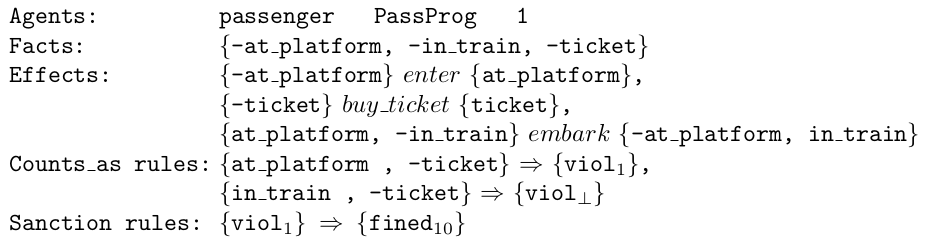
\includegraphics[width=0.8\linewidth]{figure/programdastani.png} 
  \caption{Um programa descrito na linguagem proposta neste estudo onde um agente representa um passageiro em uma estação de trem que pode entrar com ou sem um \textit{ticket} na plataforma e no trem \cite{dastaniframework}.}
  \label{exemploprograma}
\end{figure}


A Figura \ref{exemploprograma} apresenta um programa que contem um agente com nome \textit{passenger}. O agente pode estar ou não na plataforma e no trem, sem ou com \textit{ticket}. Se o agente entrar na plataforma ou no trem sem o \textit{ticket}, então esse agente cometeu uma violação. Para este programa, a sanção da violação que ocorre por entrar na plataforma sem o \textit{ticket} resulta em uma punição onde o agente deve pagar 10 Euros pelo ocorrido \cite{dastaniframework}.
